\subsection{Editar una ley de lex.gal}

La principal funcionalidad de esta aplicación es la de editar una ley de lex.gal. En esta, un usuario estará visualizando una ley de lex.gal, y procederá a editar sus datos, así como los de las leyes vinculadas. Una vez se ha realizado la edición, el usuario ha de guardar sus cambios, y estos han de ser almacenados en la base de datos.

\begin{figure}[H]
\centerline{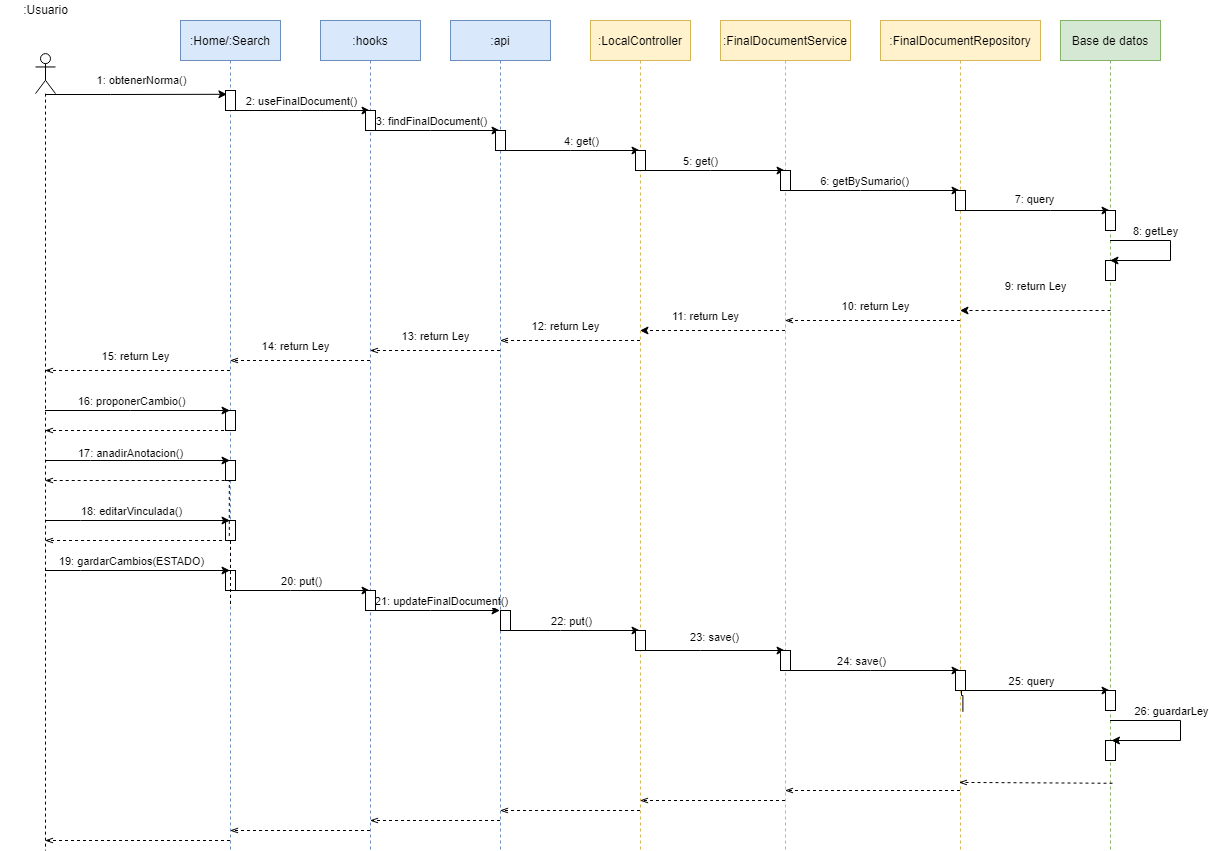
\includegraphics[width=15cm]{figuras/diseño/EditarLey.png}}
\caption{Diagrama de secuencia 03. Editar una ley de lex.gal.}
\label{enlaceDEditar}
\end{figure}

En la \hyperref[enlaceDRegistro]{Figura 3.10} se ilustra el diagrama de secuencia de la operación de edición de una ley de lex.gal. Se puede resumir en los siguientes pasos:

\begin{enumerate}
    \item El usuario entra en la página de edición de una ley, llamando al método que invoca al hook.
    \item Este método invoca al hook useFinalDocument() del archivo contenido en hooks().
    \item Se invoca al método findFinalDocument() de la carpeta {\bf api}.
    \item Se hace un llamamiento mediante una solicitud HTTP al servidor. En concreto, la función get() de LocalController, pues se hace un GET.
    \item Se invoca al servicio get() de FinalDocumentService.
    \item Se invoca la operación getBySumario() del repositorio FinalDocumentRepository, pues se busca según el sumario.
    \item Se invoca la operación de recuperar en la base de datos de MongoDB.
    \item Se recupera la leyes encontrada en la base de datos.
    \item Se procede a devolver la respuesta al usuario desde este paso, realizando el proceso inverso. El usuario recibirá las ley correspondiente. Se realiza este proceso {\bf hasta la operación 15}.
    \item El usuario propone cambios que se almacenan en el Store de React.
    \item El usuario añade anotaciones que se almacenan en el Store de React.
    \item El usuario propone cambios en leyes vinculadas que se almacenan en el Store de React.
    \item El usuario guarda los cambios. En función de si valida y publica, o guarda como borrador, tendrá un estado u otro.
    \item Este método invoca al método put() del hook useFinalDocument().
    \item Se invoca al método updateFinalDocument() de la carpeta  {\bf api}.
    \item Se hace un llamamiento mediante una solicitud HTTP al servidor. En concreto, la función put() de LocalController, pues se hace un PUT.
    \item Se invoca al servicio save() de FinalDocumentService.
    \item Se invoca la operación save() del repositorio FinalDocumentRepository, para poder modificar una ley.
    \item Se invoca la operación de modificación en la base de datos de MongoDB.
    \item Se modifica la ley correspondiente en la base de datos.
    \item Se procede a devolver la respuesta al usuario desde este paso, realizando el proceso inverso. El usuario recibirá un mensaje de que la operación fue satisfactoria.
\end{enumerate}